%%%%%%%%%%%%%%%%%%%%%%%%%%%%%%%%%%%%%%%%%
% Beamer Presentation
% LaTeX Template
% Version 1.0 (10/11/12)
%
% This template has been downloaded from:
% http://www.LaTeXTemplates.com
%
% License:
% CC BY-NC-SA 3.0 (http://creativecommons.org/licenses/by-nc-sa/3.0/)
%
%%%%%%%%%%%%%%%%%%%%%%%%%%%%%%%%%%%%%%%%%

%----------------------------------------------------------------------------------------
%	PACKAGES AND THEMES
%----------------------------------------------------------------------------------------

\documentclass{beamer}

\mode<presentation> {

% The Beamer class comes with a number of default slide themes
% which change the colors and layouts of slides. Below this is a list
% of all the themes, uncomment each in turn to see what they look like.

%\usetheme{default}
%\usetheme{AnnArbor}
%\usetheme{Antibes}
%\usetheme{Bergen}
%\usetheme{Berkeley}
%\usetheme{Berlin}
%\usetheme{Boadilla}
%\usetheme{CambridgeUS}
%\usetheme{Copenhagen}
\usetheme{Darmstadt}		% hodne dobry
%\usetheme{Dresden}			% dobry
%\usetheme{Frankfurt}
%\usetheme{Goettingen}
%\usetheme{Hannover}
%\usetheme{Ilmenau}
%\usetheme{JuanLesPins}
%\usetheme{Luebeck}
%\usetheme{Madrid}
%\usetheme{Malmoe}			
%\usetheme{Marburg}
%\usetheme{Montpellier}
%\usetheme{PaloAlto}
%\usetheme{Pittsburgh}
%\usetheme{Rochester}
%\usetheme{Singapore}			
%\usetheme{Szeged}
%\usetheme{Warsaw}		% dobry

% As well as themes, the Beamer class has a number of color themes
% for any slide theme. Uncomment each of these in turn to see how it
% changes the colors of your current slide theme.

%\usecolortheme{albatross}
%\usecolortheme{beaver}			% cerveny
%\usecolortheme{beetle}
%\usecolortheme{crane}		% oranzova
%\usecolortheme{dolphin}		%modra
%\usecolortheme{dove}		
%\usecolortheme{fly}
%\usecolortheme{lily}			
\usecolortheme{orchid}		% tmave modra a cerna
%\usecolortheme{rose}		% tmave modra a svetle bloky
%\usecolortheme{seagull}
%\usecolortheme{seahorse}		% svetle modra
%\usecolortheme{whale}
%\usecolortheme{wolverine}

%\setbeamertemplate{footline} % To remove the footer line in all slides uncomment this line
%\setbeamertemplate{footline}[page number] % To replace the footer line in all slides with a simple slide count uncomment this line

%\setbeamertemplate{navigation symbols}{} % To remove the navigation symbols from the bottom of all slides uncomment this line
}

\usepackage[utf8]{inputenc}	% kódování textu
\usepackage[czech]{babel}		% zavedení češtiny
\usepackage{amsmath,amsfonts,amssymb}	% matematika
\usepackage{graphicx} % Allows including images
\usepackage{booktabs} % Allows the use of \toprule, \midrule and \bottomrule in tables
\usepackage{multirow}	% slouceni radek v tabulce
\usepackage{multicol}	% slouceni sloupcu v tabulce
\usepackage{longtable}	% rozdeleni tabulky pres vice stran
\usepackage{enumerate}	% seznamy
\usepackage{float}
\usepackage{lscape}		% stranka na sirku
\usepackage{fancyhdr}
\usepackage{url}
\usepackage{array}
\usepackage{subfigure}
\usepackage{dirtree}
\usepackage{setspace}
\usepackage{color}
\usepackage{listings}
\usepackage{multimedia}

\AtBeginSection[]{
  \begin{frame}
  \vfill
  \centering
  \begin{beamercolorbox}[sep=8pt,center,shadow=true,rounded=true]{title}
    \usebeamerfont{title}\insertsectionhead\par%
  \end{beamercolorbox}
  \vfill
  \end{frame}
}


%------------------------------------------------------------------
%	TITLE PAGE
%------------------------------------------------------------------

\title[QGIS VFK Plugin Improvements]{Rozšíření nástroje pro práci s~katastrálními daty v~programu QGIS} % The short title appears at the bottom of every slide, the full title is only on the title page

\author{Bc. Štěpán Bambula} % Your name
\institute[ČVUT] % Your institution as it will appear on the bottom of every slide, may be shorthand to save space
{
České vysoké učení technické v Praze \\ % Your institution for the title page
%\medskip
Fakulta stavební \\
%\medskip
Obor Geomatika
% \textit{stepan.bambula@fsv.cvut.cz} % Your email address
}
\date{18. června 2016} % Date, can be changed to a custom date
\titlegraphic{
\includegraphics[width=1.5cm]{images/logoCVUT.pdf}}

\begin{document}

\begin{frame}
\titlepage % Print the title page as the first slide
\end{frame}

\begin{frame}
\frametitle{Obsah} % Table of contents slide, comment this block out to remove it
\tableofcontents % Throughout your presentation, if you choose to use \section{} and \subsection{} commands, these will automatically be printed on this slide as an overview of your presentation
\end{frame}

%------------------------------------------------------------------
%	PRESENTATION SLIDES
%------------------------------------------------------------------

%------------------------------------------------
\section{Teoretický úvod} % Sections can be created in order to organize your presentation into discrete blocks, all sections and subsections are automatically printed in the table of contents as an overview of the talk
%------------------------------------------------
\subsection{Zadání} % A subsection can be created just before a set of slides with a common theme to further break down your presentation into chunks

\begin{frame}
\frametitle{Zadání diplomové práce}

\begin{block}{Rozšíření stávajícího zásuvného modulu:}
  \begin{itemize}
    \item Usnadnění distribuce zásuvného modulu.
    \item Zpracování a vizualizace změnových vět souborů VFK.
    \item Doplnění o další vhodné funkcionality.
  \end{itemize}
\end{block}

\end{frame}

%------------------------------------------------------------------

\subsection{Použité technologie} % A subsection can be created just before a set of slides with a common theme to further break down your presentation into chunks

\begin{frame}
\frametitle{Použité technologie}
  \begin{figure}
    \centering
    \begin{minipage}{.5\textwidth}
      \centering
      \visible<1->{
	\begin{figure}[ht]
	  
\includegraphics[width=4cm]{images/qgis-logo.png}
	\end{figure}
      }
    \end{minipage}%
    \begin{minipage}{.5\textwidth}
      \centering
      \visible<2->{
	\begin{figure}[ht]
	    
\includegraphics[width=2cm]{images/gdal-logo.png}
	\end{figure}
      }
    \end{minipage}
  \end{figure}

  \begin{figure}
    \centering
    \begin{minipage}{.5\textwidth}
      \centering
      \visible<3->{
	\begin{figure}[ht]
	  
\includegraphics[width=5cm]{images/python-logo.png}
	\end{figure}
      }
    \end{minipage}%
    \begin{minipage}{.5\textwidth}
      \centering
      \visible<4->{
	\begin{figure}[ht]
	  
\includegraphics[width=2cm]{images/pyqt-logo.png}
	\end{figure}
      }
    \end{minipage}
  \end{figure}
\end{frame}

%------------------------------------------------------------------

\subsection{Informační systém katastru nemovitostí}

\begin{frame}
\frametitle{Informační systém katastru nemovitostí}

\begin{itemize}
 \item V provozu od září roku 2001,
 \item současné vedení SPI a SGI,
 \item integruje vedení a správu katastru nemovitostí pod jediný informační systém,
 \item data uložena v centrální databázi Oracle,
 \item historizace dat.
\end{itemize}

\end{frame}

%------------------------------------------------------------------

\begin{frame}
 \frametitle{Poskytování dat z ISKN}
 



\begin{columns}[onlytextwidth]
  \begin{column}{0.4\textwidth}
  
    \begin{itemize}
      \item Nahlížení do KN,
      \item Dálkový přístup do KN,
      
      \hspace{30pt}\vdots
      
      \item výměnný formát ISKN.      
    \end{itemize}
    
  \end{column}
  
  \begin{column}{0.6\textwidth}
    \begin{figure}
      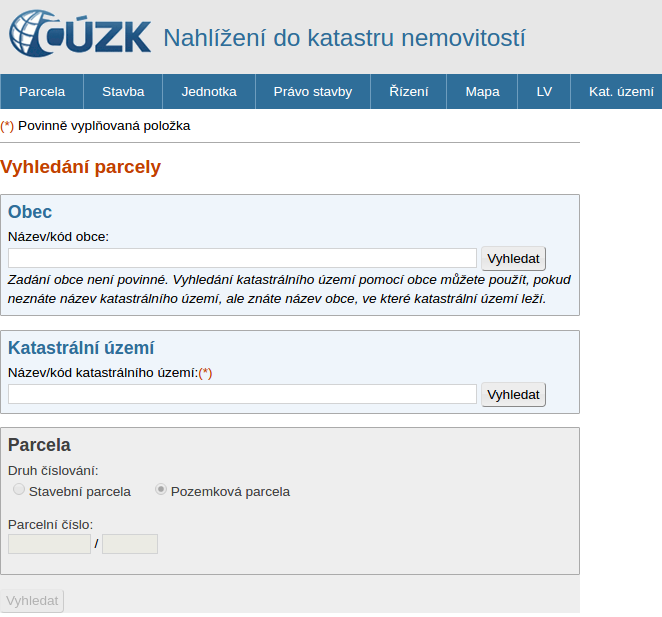
\includegraphics[width=1\textwidth]{images/nahlizeniDoKN.png}
    \end{figure}
  \end{column}

\end{columns}

\end{frame}

%------------------------------------------------------------------

\begin{frame}
\frametitle{Výměnný formát ISKN}

\begin{itemize}
  \item Zároveň popisné i grafické informace včetně dat o~řízení,
  \item stavová vs. změnová data,
  \item poskytována v rozsahu:
  
  \begin{itemize}
  \item územní jednotka,
  \item oprávněný subjekt,
  \item výběr parcel,
  \item výběr parcel polygonem v mapě.
  \end{itemize}

\item datové skupiny:

  \begin{itemize}
    \item nemovitosti, jednotky, bonitní díly parcel, vlastnictví, jiné právní vztahy, \dots
  \end{itemize}
  
\end{itemize}

\end{frame}

%------------------------------------------------------------------

\begin{frame}
\frametitle{Struktura VFK}
 
\begin{itemize}
  \item Části datového souboru:
  
  \begin{itemize}
    \item hlavička \textit{\&H},
    \item datové bloky \textit{\&D},
    \item koncový znak \textit{\&K},
  \end{itemize}
  
  \item jednotlivé záznamy odděleny středníkem.

\end{itemize}

\end{frame}

%------------------------------------------------------------------

\section{Úprava VFK ovladače v knihovně GDAL}

\subsection{Načítání dat z více souborů}

\begin{frame}
\frametitle{Načítání dat z více souborů}

\begin{columns}%[onlytextwidth]
  \begin{column}{0.5\textwidth}
  
    \begin{itemize}
     \item Ukládání dat do již existující databáze SQLite,
     \item porovnání tabulek s datovými bloky,
     \item kontrola duplicit: změnový vs. stavový soubor.
    \end{itemize}
    
  \end{column}
  
  \begin{column}{0.4\textwidth}
  Struktura uložení:
    \dirtree{%
    .1 /.
    .2 nemodebo.
    .3 vfk\_soubor.vfk.
    .2 nvfpkmbpej.
    .3 vfk\_soubor.vfk.
    .2 \vdots.
    }
  \end{column}

\end{columns}
  
\end{frame}

%------------------------------------------------------------------

\subsection{Vytváření geometrie prvků}

\begin{frame}
\frametitle{Vytváření geometrie prvků}

Dosavadní chování:
\begin{itemize}
 \item Geometrie sestavena při požadavku o konkrétní prvek,
  \begin{itemize}
   \item např. \texttt{ogrinfo vfk\_soubor.vfk PAR -FID 1}
  \end{itemize}
\end{itemize}

Nové chování:
\begin{itemize}
 \item Sestavení geometrie ihned po načtení dat do databáze.
\end{itemize}

\end{frame}

%------------------------------------------------------------------

\subsection{Čtení z databáze SQLite}

\begin{frame}
\frametitle{Čtení z databáze SQLite}

\begin{itemize}
 \item Díky již vytvořené geometrii prvků,
 \item načtení databáze po aplikaci změn.
\end{itemize}

\end{frame}

%------------------------------------------------------------------

\section{QGIS VFK Plugin -- původní verze}

\subsection{První verze zásuvného modulu VFK pro QGIS}

\begin{frame}
\frametitle{První verze zásuvného modulu VFK pro QGIS}

\begin{itemize}
 \item V jazyce C++,
 \item autoři: Václav Petráš, Anna Kratochvílová,
 \item čtení souborů VFK pomocí GDAL do databáze SQLite,
 \item struktura databáze shodná se strukturou VFK souboru.
\end{itemize}

\begin{figure}
  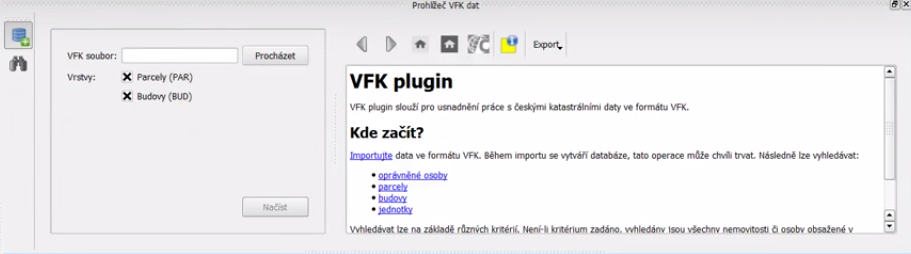
\includegraphics[width=0.9\textwidth]{images/vfkPlugin-puvodni.png}
\end{figure}

\end{frame}

%------------------------------------------------------------------

\begin{frame}
\frametitle{Funkcionalita VFK Pluginu}

\begin{columns}%[onlytextwidth]

  \begin{column}{0.6\textwidth}
    Vyhledávání:
    \begin{itemize}
    \item vlastníky, budovy, parcely, jednotky,
    \item propojení s aplikací \textit{Nahlížení do katastru nemovitostí}.
    \end{itemize}

    Export výsledků:
    \begin{itemize}
    \item HTML, \LaTeX.
    \end{itemize}

    Interakce s mapovým oknem QGIS:
    \begin{itemize}
    \item výběr nástrojem QGIS, zobrazení vyhledaných prvků.
    \end{itemize}   
    
  \end{column}
  
  \begin{column}{0.4\textwidth}
    \begin{figure}
      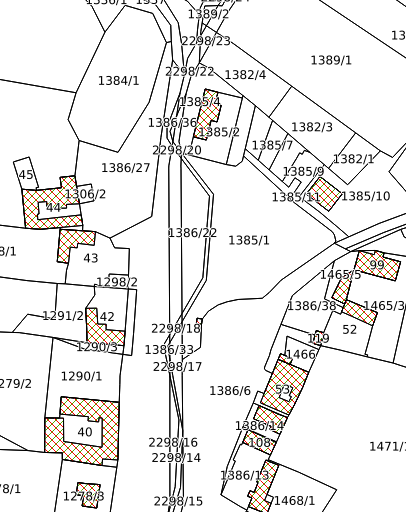
\includegraphics[width=1\textwidth]{images/vfkPlugin-nactena_data.png}
    \end{figure}
  \end{column}

\end{columns}

\end{frame}

%------------------------------------------------------------------
\section{Nově přidané funkcionality}

\subsection{Usnadnění distribuce zásuvného modulu}

\begin{frame}
\frametitle{Usnadnění distribuce zásuvného modulu}

\begin{itemize}
 \item Nevýhody C++ verze:
 
 \begin{itemize}
  \item komplikovaná instalace / aktualizace.
 \end{itemize}
 
 \item Přepis do jazyka Python:
 
 \begin{itemize}
  \item vygenerování struktury pluginu pomocí nástroje \textit{Plugin Builder},
  \item použití shodných knihoven,
  \item instalace ze vzdáleného repositáře QGIS (\url{http://geo.fsv.cvut.cz/osgeorel/qgis-plugins.xml}),
  \item dostupný v oddělené vývojové větvi.
 \end{itemize}

\end{itemize}

\end{frame}

%------------------------------------------------------------------

\begin{frame}
\frametitle{Instalace zásuvného modulu}

\begin{figure}
  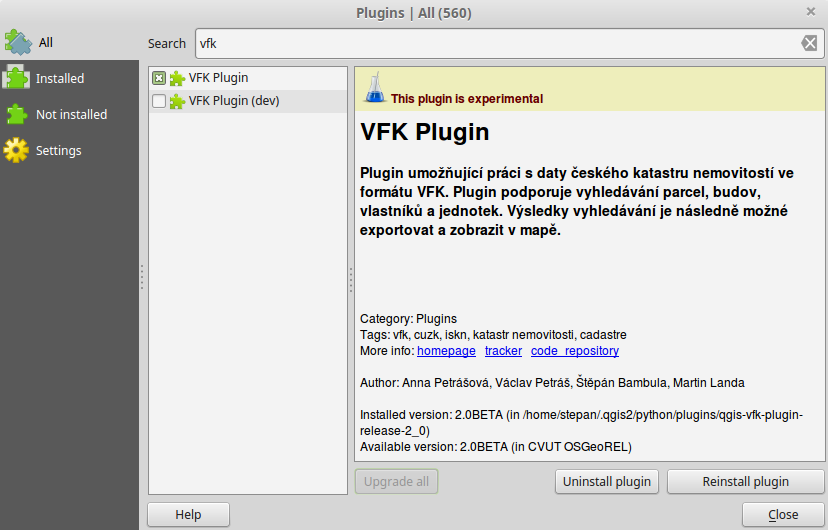
\includegraphics[width=.9\textwidth]{images/qgis_plugin_vyhledani.png}
\end{figure}

\end{frame}

%------------------------------------------------------------------

\subsection{Zpracování změnových vět}

\begin{frame}
\frametitle{Změnové věty ve VFK}

\begingroup 
  \fontsize{8pt}{12pt}\selectfont


\begin{table}[htbp]
\centering
\begin{tabular}{lccl}
\toprule
\textbf{Operace} & \textbf{\parbox{20pt}{Stav dat}} & \textbf{\parbox{30pt}{Kontext změn}} & \textbf{Událost} \\ \midrule
\multirow{3}{*}{UPDATE} & -1 & 1 & \parbox{150pt}{Objekt byl změněn, původní verze zanikla, nová verze vznikla (záznam je v~minulosti).} \vspace{6pt} \\ 
 & -1 & 3 & \parbox{150pt}{Objekt vznikl a později byl změněn. Verze není vzhledem k~sys. datu aktuální, (záznam je v~minulosti).} \vspace{6pt} \\ 
 & 0 & 3 & \parbox{150pt}{Objekt byl změněn. Nová verze je vzhledem k~sys. datu aktuální.} \vspace{6pt} \\ 
DELETE & 3 & 1 & \parbox{150pt}{Objekt byl v~exportovaném období zrušen.} \vspace{6pt} \\ 
INSERT & 0 & 3 & \parbox{150pt}{Objekt vznikl v~exportovaném období.} \vspace{6pt} \\ 
LOCK & 0 & 2 & \parbox{150pt}{Objekty zadané ve vstupních parametrech.} \\ \bottomrule
\end{tabular}
\end{table}

\endgroup
\end{frame}

%------------------------------------------------------------------

\begin{frame}
\frametitle{Načítání změnových souborů}

\begin{columns}%[onlytextwidth]

  \begin{column}{0.5\textwidth}

    \begin{itemize}
    \item Stejná struktura jako stavová data,
    \item nutné změny ve čtení souborů na straně VFK ovladače GDAL i VFK Pluginu.
    \end{itemize}
  
  \end{column}
  
  \begin{column}{0.5\textwidth}
  
    \begin{figure}
      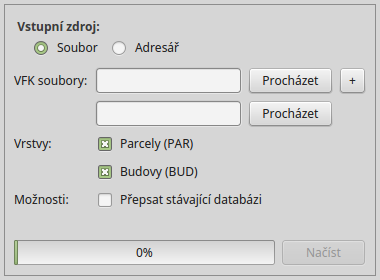
\includegraphics[width=.9\textwidth]{images/vfkPlugin-nacitani.png}
    \end{figure}
    
  \end{column}

\end{columns}

\end{frame}

%------------------------------------------------------------------

\begin{frame}
\frametitle{Aplikace změn}

\begin{columns}%[onlytextwidth]

  \begin{column}{0.5\textwidth}

    \begin{itemize}
      \item Pracuje s databázemi SQLite,
      \item samostatná třída použitelná i jako konzolová aplikace,
      \item ikona aplikace změn:
    \end{itemize}
    
    \begin{figure}
      
\includegraphics[scale=.8]{images/zmeny_ikona.png}
    \end{figure}
  
  \end{column}
  
  \begin{column}{0.5\textwidth}
  
    \begin{figure}
      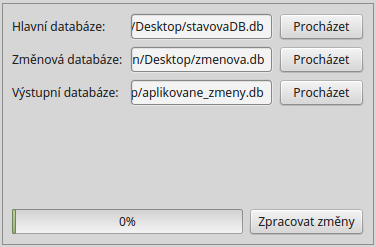
\includegraphics[width=.9\textwidth]{images/vfkPlugin-zmeny.png}
    \end{figure}
    
  \end{column}

\end{columns}

\end{frame}

%------------------------------------------------------------------

\begin{frame}[fragile]
\frametitle{Konzolová aplikace -- nápověda}

\begin{scriptsize}
\begin{lstlisting}[moredelim={[is][keywordstyle]{@@}{@@}}]
@@$ ./applyChanges.py -h @@

Usage: applyChanges.py [-h] [-v] -i INPUT -c CHANGES 
				 -o OUTPUT [-d]

Script applies changes from amendment VFK database to main 
VFK database. In this process new database is created.

optional arguments:
  -h, --help            Show this help message and exit
  -v, --version         Show program's version number and exit
  -i INPUT, --input INPUT
                        Path to the main database.
  -c CHANGES, --changes CHANGES
                        Path to the database with changes.
  -o OUTPUT, --output OUTPUT
                        Path to the new database which will 
                        be created.
  -d, --debug           Enables debug mode.
\end{lstlisting}
\end{scriptsize}

\end{frame}

%------------------------------------------------------------------

\begin{frame}
\frametitle{Metodika aplikace změn}

\begin{enumerate}
 \item Kopie databáze se stavovými daty,
 \item hledání tabulek obsahující změny,
 \item mazání neaktuálních dat,
 \item import aktuálních dat.
\end{enumerate}

\end{frame}

%------------------------------------------------------------------

\subsection{Další nově přidané funkcionality}

\begin{frame}
\frametitle{Další nově přidané funkcionality (I)}

\textbf{Čtení z databáze SQLite:}
\begin{itemize}
 \item umožňuje načítání databáze s aplikovanými změnami,
 \item užitečné při práci s objemnými daty.
\end{itemize}

\textbf{Načítání více souborů:}
\begin{itemize}
 \item načítání do jedné databáze SQLite,
 \item načítání omezeno na pět souborů.
\end{itemize}

\textbf{Načítání VFK souborů z adresáře:}
\begin{itemize}
 \item vhodné při načítání více souborů VFK,
 \item stromové procházení podadresářů.
\end{itemize}

\end{frame}

%------------------------------------------------------------------

\begin{frame}
\frametitle{Další nově přidané funkcionality (II)}


\textbf{Automatické pojmenování databáze:}
\begin{itemize}
 \item umístěna v kořenovém adresáři,
 \item pojmenování podle typu vstupního VFK souboru.
\end{itemize}

\textbf{Přepsání existující databáze:}
\begin{itemize}
 \item např. kvůli nekompatibilitě databáze s verzí GDAL,
 \item přepsání pomocí interní proměnné knihovny GDAL.
\end{itemize}

\end{frame}

%------------------------------------------------------------------

\subsection{Shrnutí}

\begin{frame}
\frametitle{Nový vzhled VFK Pluginu}

\begin{figure}
  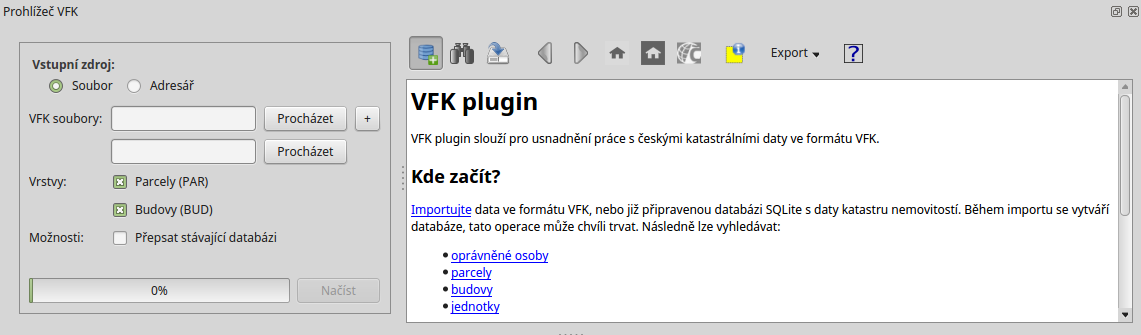
\includegraphics[width=1\textwidth]{images/vfkPlugin-novy_vzhled.png}
\end{figure}
\end{frame}

%------------------------------------------------------------------

\begin{frame}
\frametitle{Závěr}

Zdrojový kód dostupný na: 
\begin{itemize}
 \item \url{https://github.com/ctu-osgeorel/qgis-vfk-plugin}
\end{itemize}


Video ukázka:
\vspace{6pt}

\centering
\movie{
\includegraphics[width=0.9\textwidth]{images/video_uvod.png}}{dp-prezentace-video.mp4}

\end{frame}

%------------------------------------------------------------------

\begin{frame}
\Huge{\centerline{Děkuji za pozornost.}}
\end{frame}

%------------------------------------------------------------------

% \section{Posudky}
% 
% \subsection{Reakce na posudky}
% 
% \begin{frame}
% \frametitle{Reakce na posudky}
% 
% 
% \end{frame}


%==================================================================
\end{document} 
